% Draft captions written by C2_evaluation*.ipynb (diffusion). Overwritten on rerun.

% diffusion_aim1a_attr_k_sweep
\begin{figure}[t]
  \centering
  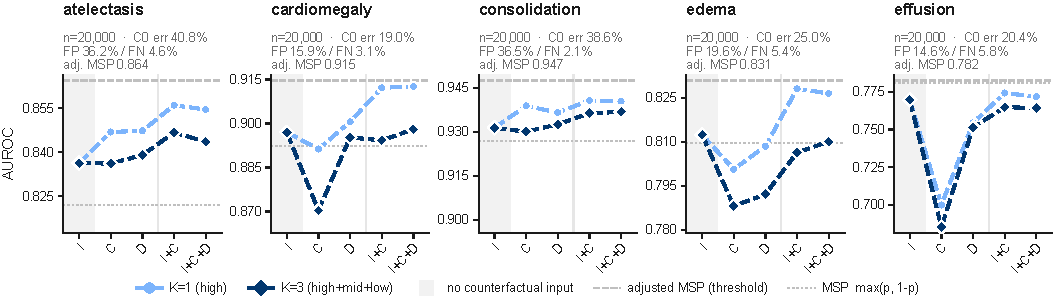
\includegraphics[width=\textwidth]{figures/c2/diffusion_aim1a_attr_k_sweep.pdf}
  \caption{Diffusion counterfactuals (FastDiME trajectories from the query), on the 20{,}000-image subset. Attribute models: mean-fold AUROC of every input configuration, one line per $K \in \{1, 3\}$. $K$ is the number of intensity levels pooled: $K=1$ is the strongest (high) edit alone, $K=3$ adds the mid and low edits. I: query attributes; C: counterfactual attributes; D: query minus counterfactual. The shaded configuration (I) sees no counterfactual, so its lines coincide across $K$. Grey lines: threshold-adjusted MSP (dashed) and plain $\max(p, 1-p)$ (dotted), the untrained baselines. Each panel has its own $y$-range.}
  \label{fig:diffusion_aim1a_attr_k_sweep}
\end{figure}

% diffusion_aim1b_attr_vs_knn
\begin{figure}[t]
  \centering
  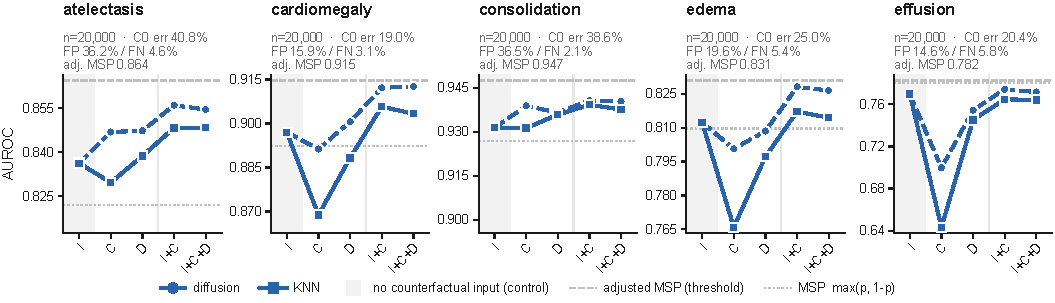
\includegraphics[width=\textwidth]{figures/c2/diffusion_aim1b_attr_vs_knn.pdf}
  \caption{Attribute models with diffusion (dashed, circles) and retrieved nearest-neighbour (solid, squares) counterfactuals, at $K = 1$. Both arms use the same 20{,}000 images, patient-grouped folds and seed, so only the source of the counterfactual differs. The shaded configuration (I) sees no counterfactual and is the control: the two arms must agree there. Grey lines: threshold-adjusted MSP (dashed) and plain $\max(p, 1-p)$ (dotted), the untrained baselines.}
  \label{fig:diffusion_aim1b_attr_vs_knn}
\end{figure}

% diffusion_aim1c_cnn_k_sweep
\begin{figure}[t]
  \centering
  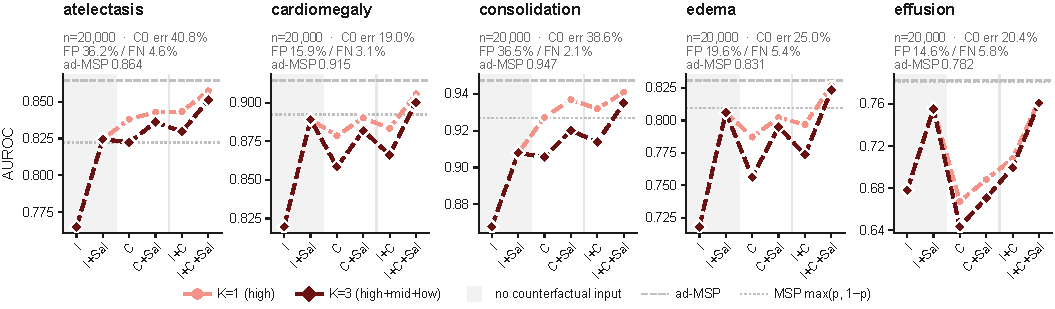
\includegraphics[width=\textwidth]{figures/c2/diffusion_aim1c_cnn_k_sweep.pdf}
  \caption{Diffusion counterfactuals (FastDiME trajectories from the query), on the 20{,}000-image subset. Image models: mean-fold AUROC of every CNN variant, one line per $K \in \{1, 3\}$. $K$ is the number of intensity levels pooled: $K=1$ is the strongest (high) edit alone, $K=3$ adds the mid and low edits. I: query image; C: counterfactual image; Sal: saliency maps; I+C uses one encoder per image. The shaded models see no counterfactual, so their lines coincide across $K$. Grey lines: threshold-adjusted MSP (dashed) and plain $\max(p, 1-p)$ (dotted), the untrained baselines. Each panel has its own $y$-range.}
  \label{fig:diffusion_aim1c_cnn_k_sweep}
\end{figure}

% diffusion_aim1d_cnn_vs_knn
\begin{figure}[t]
  \centering
  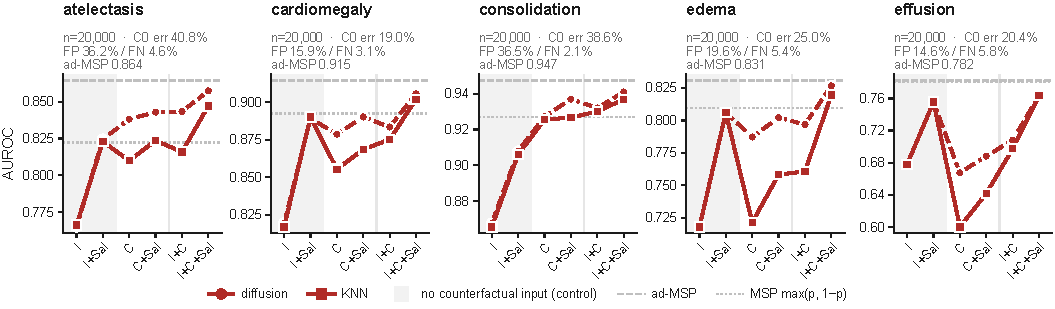
\includegraphics[width=\textwidth]{figures/c2/diffusion_aim1d_cnn_vs_knn.pdf}
  \caption{Image models with diffusion (dashed, circles) and retrieved nearest-neighbour (solid, squares) counterfactuals, at $K = 1$. Both arms use the same 20{,}000 images, patient-grouped folds and seed, so only the source of the counterfactual differs. The shaded models (I, I+Sal) see no counterfactual and are the control: the two arms must agree there. Grey lines: threshold-adjusted MSP (dashed) and plain $\max(p, 1-p)$ (dotted), the untrained baselines.}
  \label{fig:diffusion_aim1d_cnn_vs_knn}
\end{figure}

% diffusion_aim1e_trajectory
\begin{figure}[t]
  \centering
  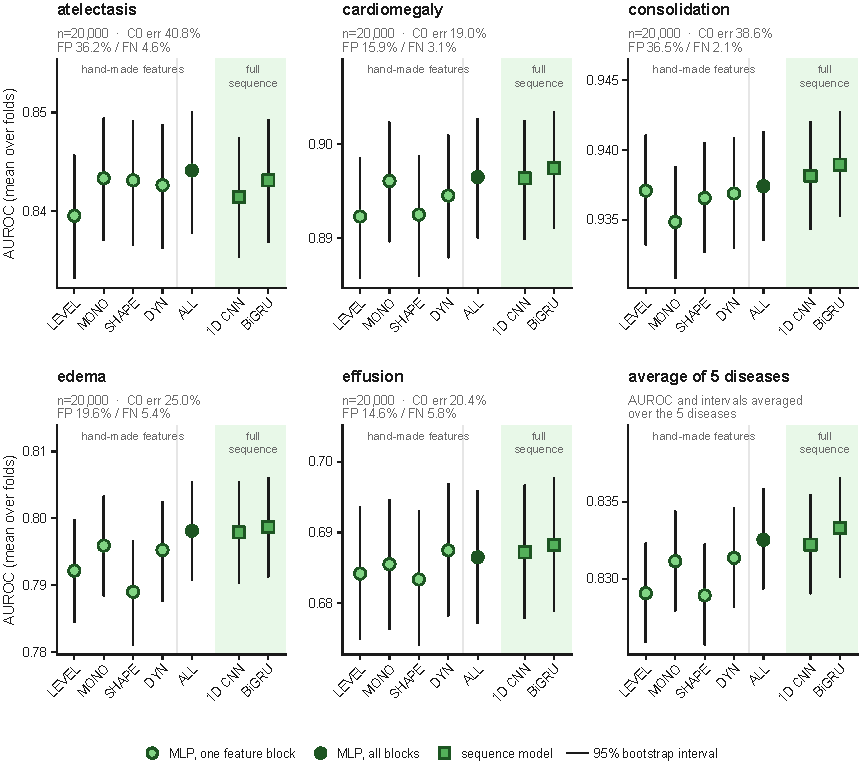
\includegraphics[width=\textwidth]{figures/c2/diffusion_aim1e_trajectory.pdf}
  \caption{Diffusion counterfactuals (FastDiME trajectories from the query), on the 20{,}000-image subset. Trajectory models, which see neither the counterfactual image nor C0's probability on the query, only C0's probability along the diffusion trajectory. Points: an MLP on each block of 32 hand-made trajectory features (LEVEL, MONO, SHAPE, DYN), sorted by AUROC within each panel, and on all of them (ALL, last); horizontal lines: a 1D CNN and a bidirectional GRU on the whole trajectory. $K = 1$. Grey lines: threshold-adjusted MSP (dashed) and plain $\max(p, 1-p)$ (dotted), the untrained baselines.}
  \label{fig:diffusion_aim1e_trajectory}
\end{figure}

% diffusion_aim1f_attr_blocks_bars
\begin{figure}[t]
  \centering
  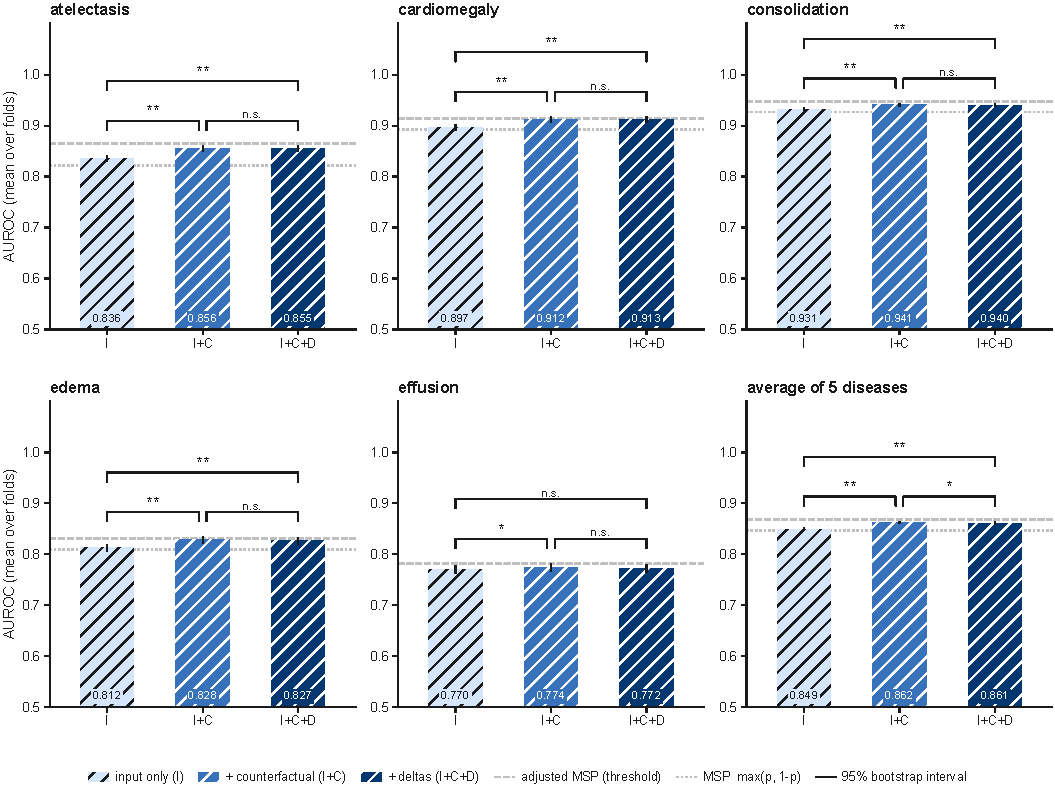
\includegraphics[width=\textwidth]{figures/c2/diffusion_aim1f_attr_blocks_bars.pdf}
  \caption{Diffusion counterfactuals (FastDiME trajectories from the query), on the 20{,}000-image subset. Adding the counterfactual to the attribute model, at $K = 1$. Bars: mean-fold AUROC of the query alone (I), with the counterfactual (I+C) and with the explicit deltas (I+C+D); whiskers: 95\% bootstrap interval of each AUROC. Brackets: paired patient-level bootstrap (5{,}000 replicates) of the mean-fold AUROC difference, Holm-adjusted across the 5 diseases (disease panels) or across the 9 claims (average panel); ***~$p_\mathrm{adj} < 0.001$, **~$p_\mathrm{adj} < 0.01$, *~$p_\mathrm{adj} < 0.05$, n.s.\ otherwise. Both models are scored on the same patients, so overlapping whiskers do not imply a non-significant difference. Grey lines: threshold-adjusted MSP (dashed) and plain $\max(p, 1-p)$ (dotted), the untrained baselines.}
  \label{fig:diffusion_aim1f_attr_blocks_bars}
\end{figure}

% diffusion_aim1g_cnn_ladder_bars
\begin{figure}[t]
  \centering
  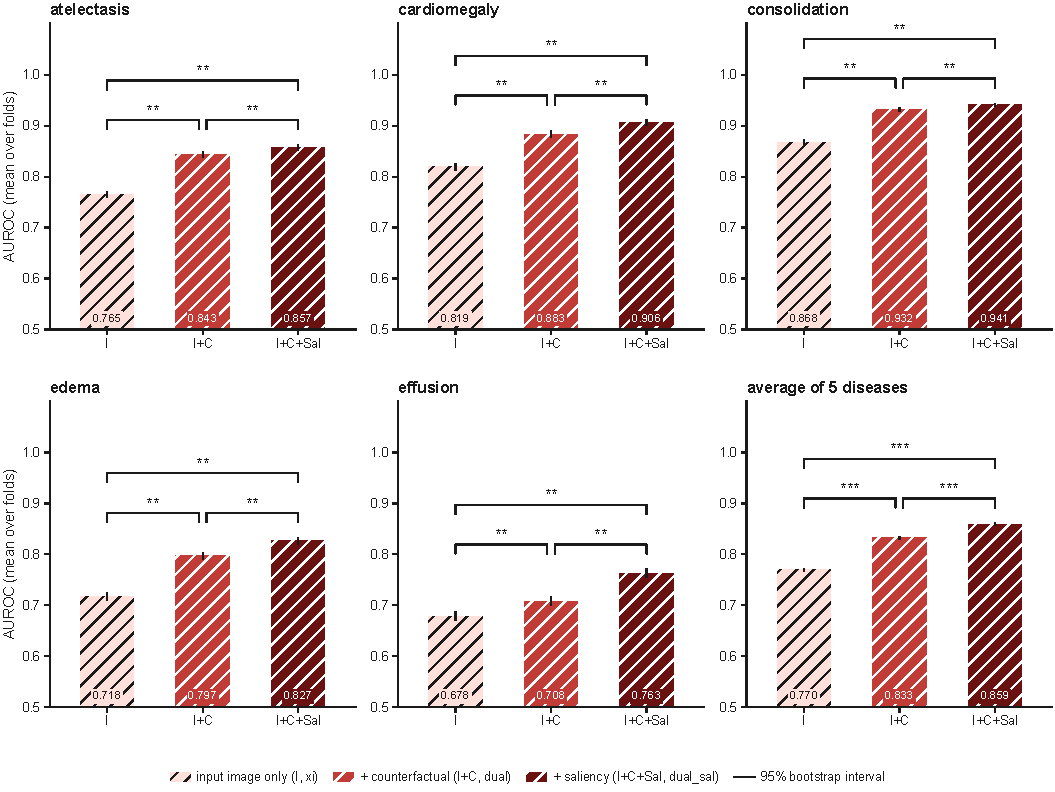
\includegraphics[width=\textwidth]{figures/c2/diffusion_aim1g_cnn_ladder_bars.pdf}
  \caption{Diffusion counterfactuals (FastDiME trajectories from the query), on the 20{,}000-image subset. Adding the counterfactual to the image model, at $K = 1$. Bars: mean-fold AUROC of the query image alone (I), with the counterfactual through a second encoder (I+C) and with both saliency maps (I+C+Sal); whiskers: 95\% bootstrap interval of each AUROC. Brackets: paired patient-level bootstrap (5{,}000 replicates) of the mean-fold AUROC difference, Holm-adjusted across the 5 diseases (disease panels) or across the 9 claims (average panel); ***~$p_\mathrm{adj} < 0.001$, **~$p_\mathrm{adj} < 0.01$, *~$p_\mathrm{adj} < 0.05$, n.s.\ otherwise. Grey lines: threshold-adjusted MSP (dashed) and plain $\max(p, 1-p)$ (dotted), the untrained baselines.}
  \label{fig:diffusion_aim1g_cnn_ladder_bars}
\end{figure}

% diffusion_aim2a_best_vs_msp
\begin{figure}[t]
  \centering
  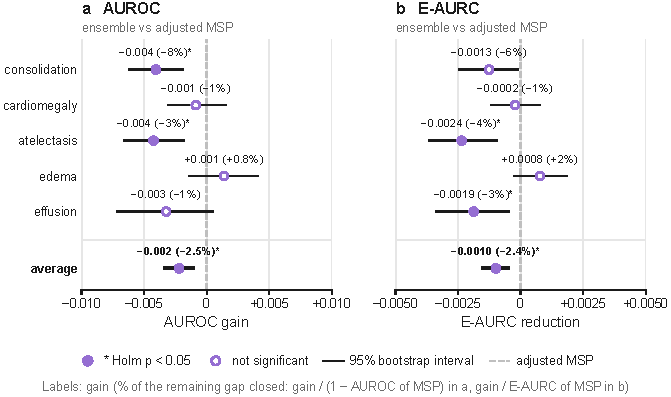
\includegraphics[width=\textwidth]{figures/c2/diffusion_aim2a_best_vs_msp.pdf}
  \caption{Diffusion counterfactuals (FastDiME trajectories from the query), on the 20{,}000-image subset.Final system against the adjusted MSP, at $K = 1$. Gain of the final system's strongest model (the ensemble in every disease) over the threshold-adjusted MSP, in mean-fold AUROC (a) and mean-fold E-AURC (b, MSP minus model, so positive is better); the dashed line is the MSP. Tasks are ordered by C0's threshold. Each label gives the gain and, in brackets, the percentage of MSP's remaining gap to a perfect ranking that it closes: $\mathrm{gain}/(1-\mathrm{AUROC}_\mathrm{MSP})$ in (a) and $\mathrm{gain}/\mathrm{E\text{-}AURC}_\mathrm{MSP}$ in (b). The average row gives the mean gain and the mean of the five per-task percentages. Whiskers: 95\% intervals of a paired patient-level bootstrap (5{,}000 replicates). Filled points and $*$: Holm-adjusted $p < 0.05$. The correction runs across the 5 tasks within each panel, separately for (a) and (b), not across all 10 tests; the AUROC average is corrected across the 9 thesis claims, the E-AURC average is a single test.}
  \label{fig:diffusion_aim2a_best_vs_msp}
\end{figure}

% diffusion_aim2a_risk_coverage
\begin{figure}[t]
  \centering
  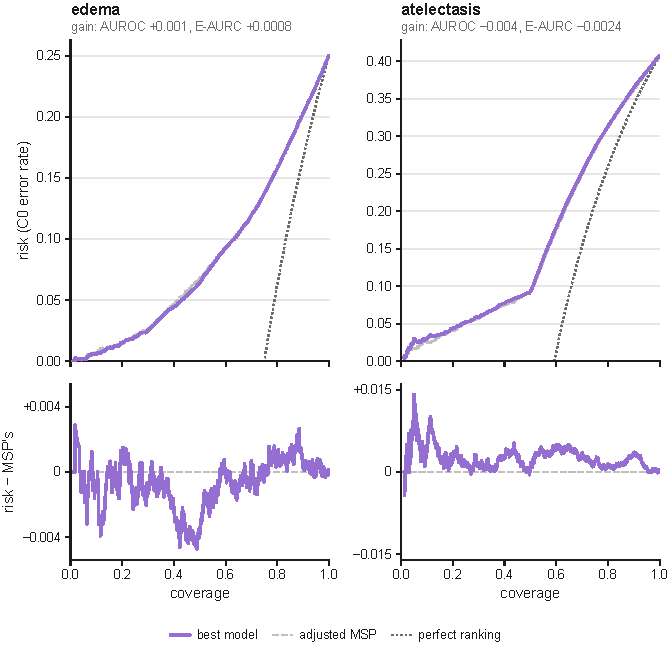
\includegraphics[width=\textwidth]{figures/c2/diffusion_aim2a_risk_coverage.pdf}
  \caption{Diffusion counterfactuals (FastDiME trajectories from the query), on the 20{,}000-image subset.Risk-coverage of the final system's strongest model against the adjusted MSP, for the tasks with the largest and smallest AUROC gain. Top: C0's error rate among the retained cases, most confident first; dotted: a perfect ranking. Bottom: the model's risk minus MSP's (below zero: fewer errors retained). Pooled out-of-fold predictions; the first 200 retained cases are not drawn.}
  \label{fig:diffusion_aim2a_risk_coverage}
\end{figure}

% diffusion_aim2b_ensemble
\begin{figure}[t]
  \centering
  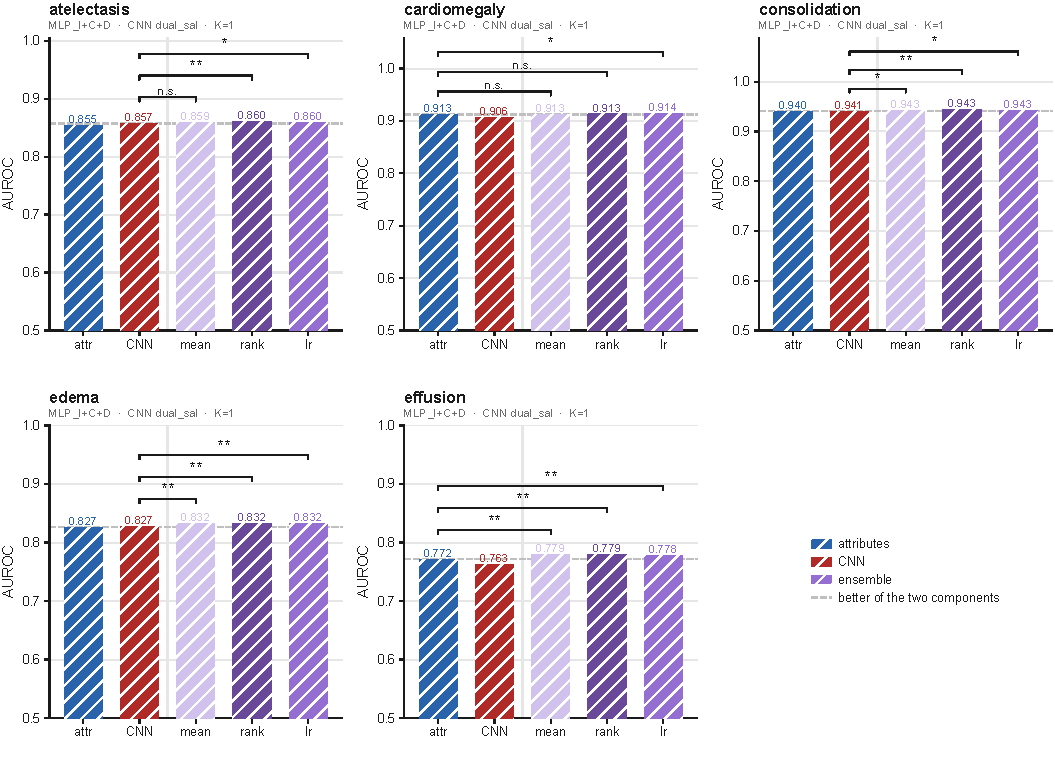
\includegraphics[width=\textwidth]{figures/c2/diffusion_aim2b_ensemble.pdf}
  \caption{Diffusion counterfactuals (FastDiME trajectories from the query), on the 20{,}000-image subset. Combining the final attribute model and CNN ($K = 1$). Bars: mean-fold AUROC of the two components and three combiners --- the mean of the two probabilities, the mean of their within-fold ranks, and a logistic regression fitted leave-one-fold-out. Dashed line: the better component. Brackets: paired patient-level bootstrap (5{,}000 replicates) of the mean-fold AUROC difference, Holm-adjusted across the 15 combiner--disease tests of the figure, of each combiner against the better component; ***~$p_\mathrm{adj} < 0.001$, **~$p_\mathrm{adj} < 0.01$, *~$p_\mathrm{adj} < 0.05$, n.s.\ otherwise.}
  \label{fig:diffusion_aim2b_ensemble}
\end{figure}

% diffusion_aim2c_arm_points
\begin{figure}[t]
  \centering
  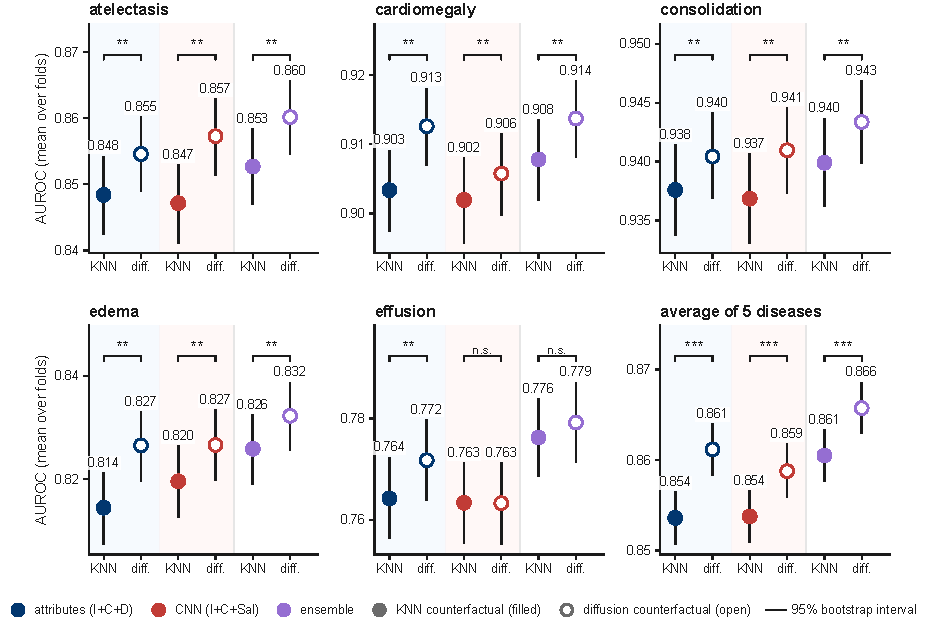
\includegraphics[width=\textwidth]{figures/c2/diffusion_aim2c_arm_points.pdf}
  \caption{The final system with retrieved nearest-neighbour (filled) and diffusion (open) counterfactuals, at $K = 1$: the attribute model (I+C+D), the CNN (I+C+Sal) and the ensemble, whose combiner is each arm's own best. Both arms use the same 20{,}000 images, patient-grouped folds and seed, so only the source of the counterfactual differs. Points: mean-fold AUROC; whiskers: 95\% bootstrap interval. Brackets: paired patient-level bootstrap (5{,}000 replicates) of the mean-fold AUROC difference, Holm-adjusted within each disease (average panel: across comparisons), diffusion against KNN; ***~$p_\mathrm{adj} < 0.001$, **~$p_\mathrm{adj} < 0.01$, *~$p_\mathrm{adj} < 0.05$, n.s.\ otherwise. The ensemble bracket compares two winners chosen after scoring. Each panel has its own $y$-range.}
  \label{fig:diffusion_aim2c_arm_points}
\end{figure}

% diffusion_aim1f_attr_blocks_points
\begin{figure}[t]
  \centering
  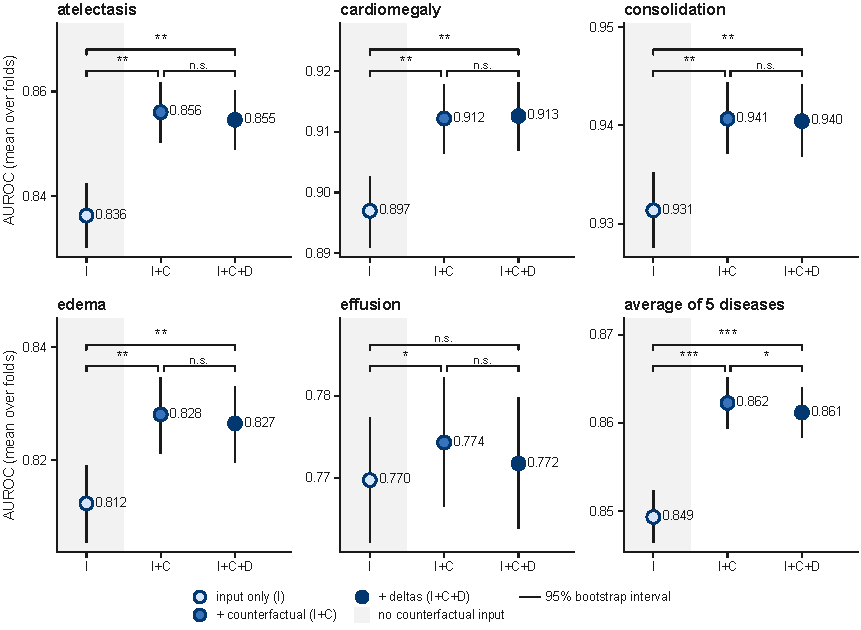
\includegraphics[width=\textwidth]{figures/c2/diffusion_aim1f_attr_blocks_points.pdf}
  \caption{Diffusion counterfactuals (FastDiME trajectories from the query), on the 20{,}000-image subset. Adding the counterfactual to the attribute model, at $K = 1$. Points: mean-fold AUROC of the query alone (I), with the counterfactual (I+C) and with the explicit deltas (I+C+D); whiskers: 95\% bootstrap interval of each AUROC. Brackets: paired patient-level bootstrap (5{,}000 replicates) of the mean-fold AUROC difference, Holm-adjusted across the 5 diseases (disease panels) or across the 9 claims (average panel); ***~$p_\mathrm{adj} < 0.001$, **~$p_\mathrm{adj} < 0.01$, *~$p_\mathrm{adj} < 0.05$, n.s.\ otherwise. Both models are scored on the same patients, so overlapping whiskers do not imply a non-significant difference. Grey lines: threshold-adjusted MSP (dashed) and plain $\max(p, 1-p)$ (dotted), the untrained baselines. Each panel has its own $y$-range, so compare models within a panel, not heights across panels; an MSP outside the range is printed in the panel corner.}
  \label{fig:diffusion_aim1f_attr_blocks_points}
\end{figure}

% diffusion_aim1g_cnn_ladder_points
\begin{figure}[t]
  \centering
  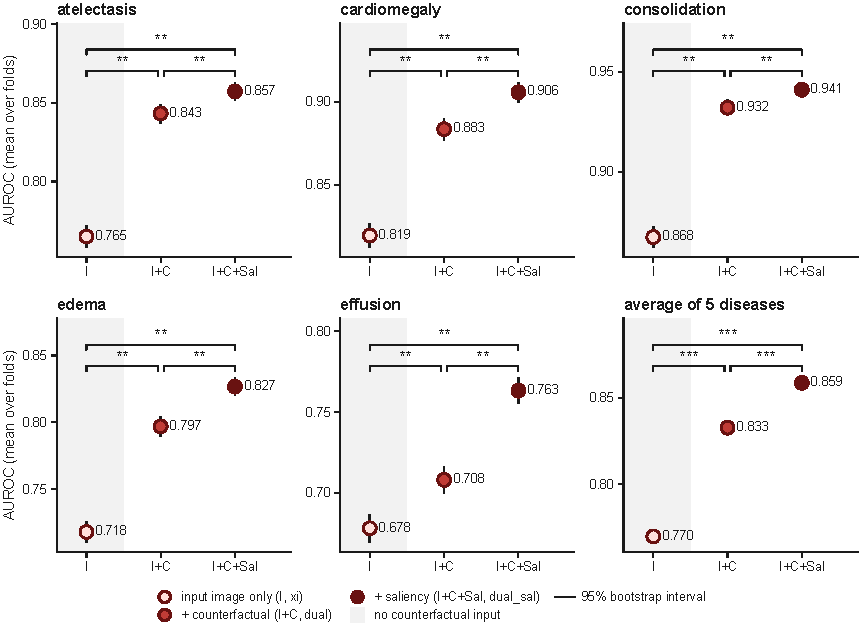
\includegraphics[width=\textwidth]{figures/c2/diffusion_aim1g_cnn_ladder_points.pdf}
  \caption{Diffusion counterfactuals (FastDiME trajectories from the query), on the 20{,}000-image subset. Adding the counterfactual to the image model, at $K = 1$. Points: mean-fold AUROC of the query image alone (I), with the counterfactual through a second encoder (I+C) and with both saliency maps (I+C+Sal); whiskers: 95\% bootstrap interval of each AUROC. Brackets: paired patient-level bootstrap (5{,}000 replicates) of the mean-fold AUROC difference, Holm-adjusted across the 5 diseases (disease panels) or across the 9 claims (average panel); ***~$p_\mathrm{adj} < 0.001$, **~$p_\mathrm{adj} < 0.01$, *~$p_\mathrm{adj} < 0.05$, n.s.\ otherwise. Grey lines: threshold-adjusted MSP (dashed) and plain $\max(p, 1-p)$ (dotted), the untrained baselines. Each panel has its own $y$-range, so compare models within a panel, not heights across panels; an MSP outside the range is printed in the panel corner.}
  \label{fig:diffusion_aim1g_cnn_ladder_points}
\end{figure}

% diffusion_aim2b_ensemble_points
\begin{figure}[t]
  \centering
  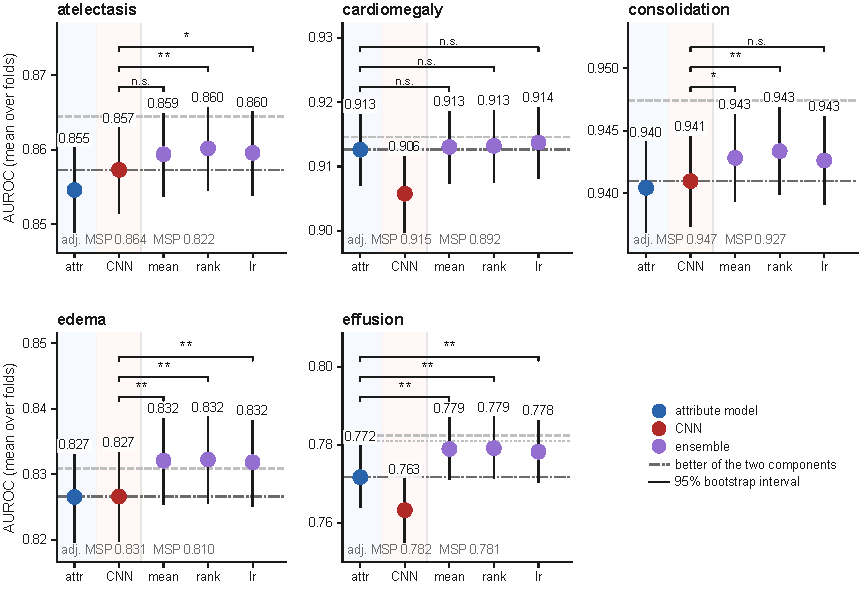
\includegraphics[width=\textwidth]{figures/c2/diffusion_aim2b_ensemble_points.pdf}
  \caption{Diffusion counterfactuals (FastDiME trajectories from the query), on the 20{,}000-image subset. Combining the final attribute model and CNN ($K = 1$). Points: mean-fold AUROC of the two components and three combiners --- the mean of the two probabilities, the mean of their within-fold ranks, and a logistic regression fitted leave-one-fold-out. Whiskers: 95\% bootstrap interval. Dash-dotted line: the better component; grey dashed and dotted lines: threshold-adjusted MSP and $\max(p, 1-p)$. Brackets: paired patient-level bootstrap (5{,}000 replicates) of the mean-fold AUROC difference, Holm-adjusted across the 15 combiner--disease tests of the figure, of each combiner against the better component; ***~$p_\mathrm{adj} < 0.001$, **~$p_\mathrm{adj} < 0.01$, *~$p_\mathrm{adj} < 0.05$, n.s.\ otherwise. Each panel has its own $y$-range, so compare models within a panel, not heights across panels; an MSP outside the range is printed in the panel corner.}
  \label{fig:diffusion_aim2b_ensemble_points}
\end{figure}
